%\clearpage
%\newgeometry{margin=0pt} % Apply margin only for this page
%\thispagestyle{empty}
%\begin{center}
%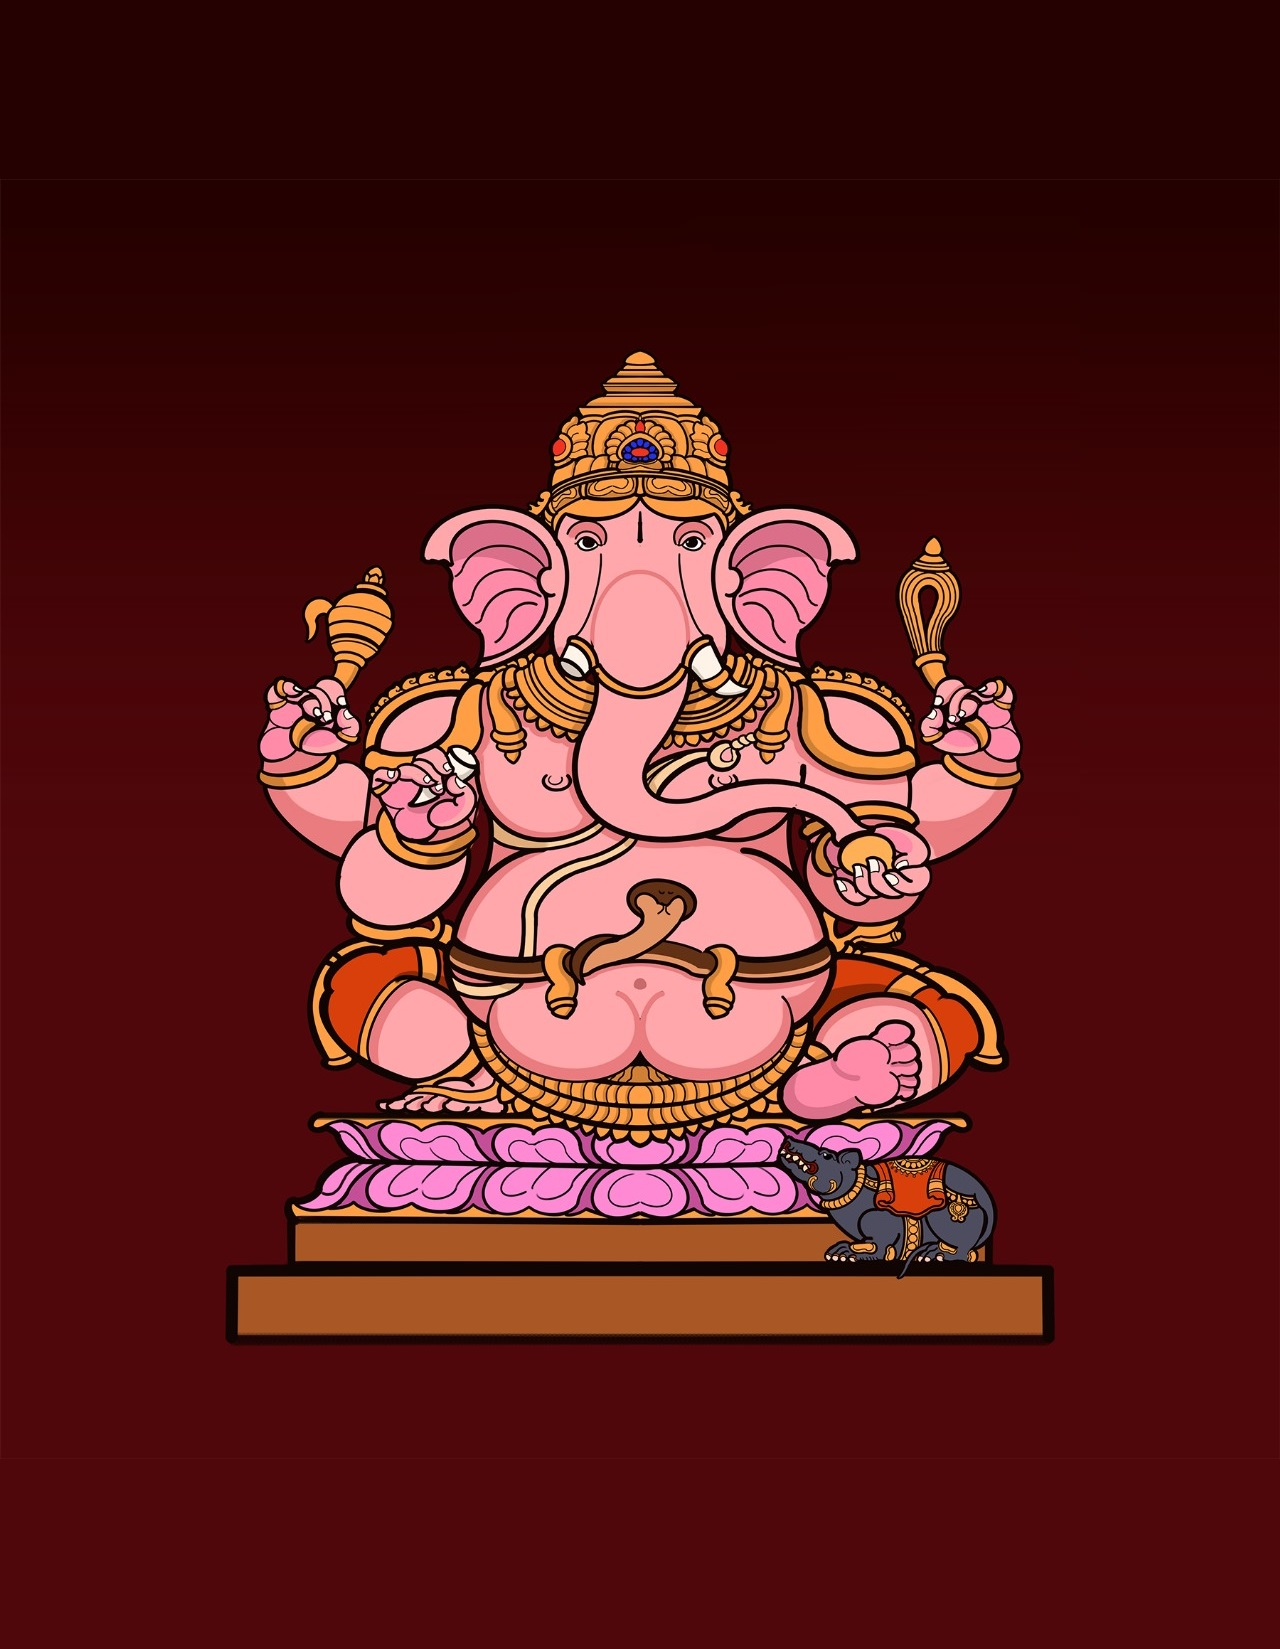
\includegraphics[width=0.9\textwidth, height=\paperheight, keepaspectratio]{./images/ganapa.jpg}
%\end{center}
%\restoregeometry % Restore original geometry settings
%\newpage

\clearpage
\newgeometry{margin=0pt} % Apply margin only for this page
\thispagestyle{empty}
%\begin{figure}
%\centering
%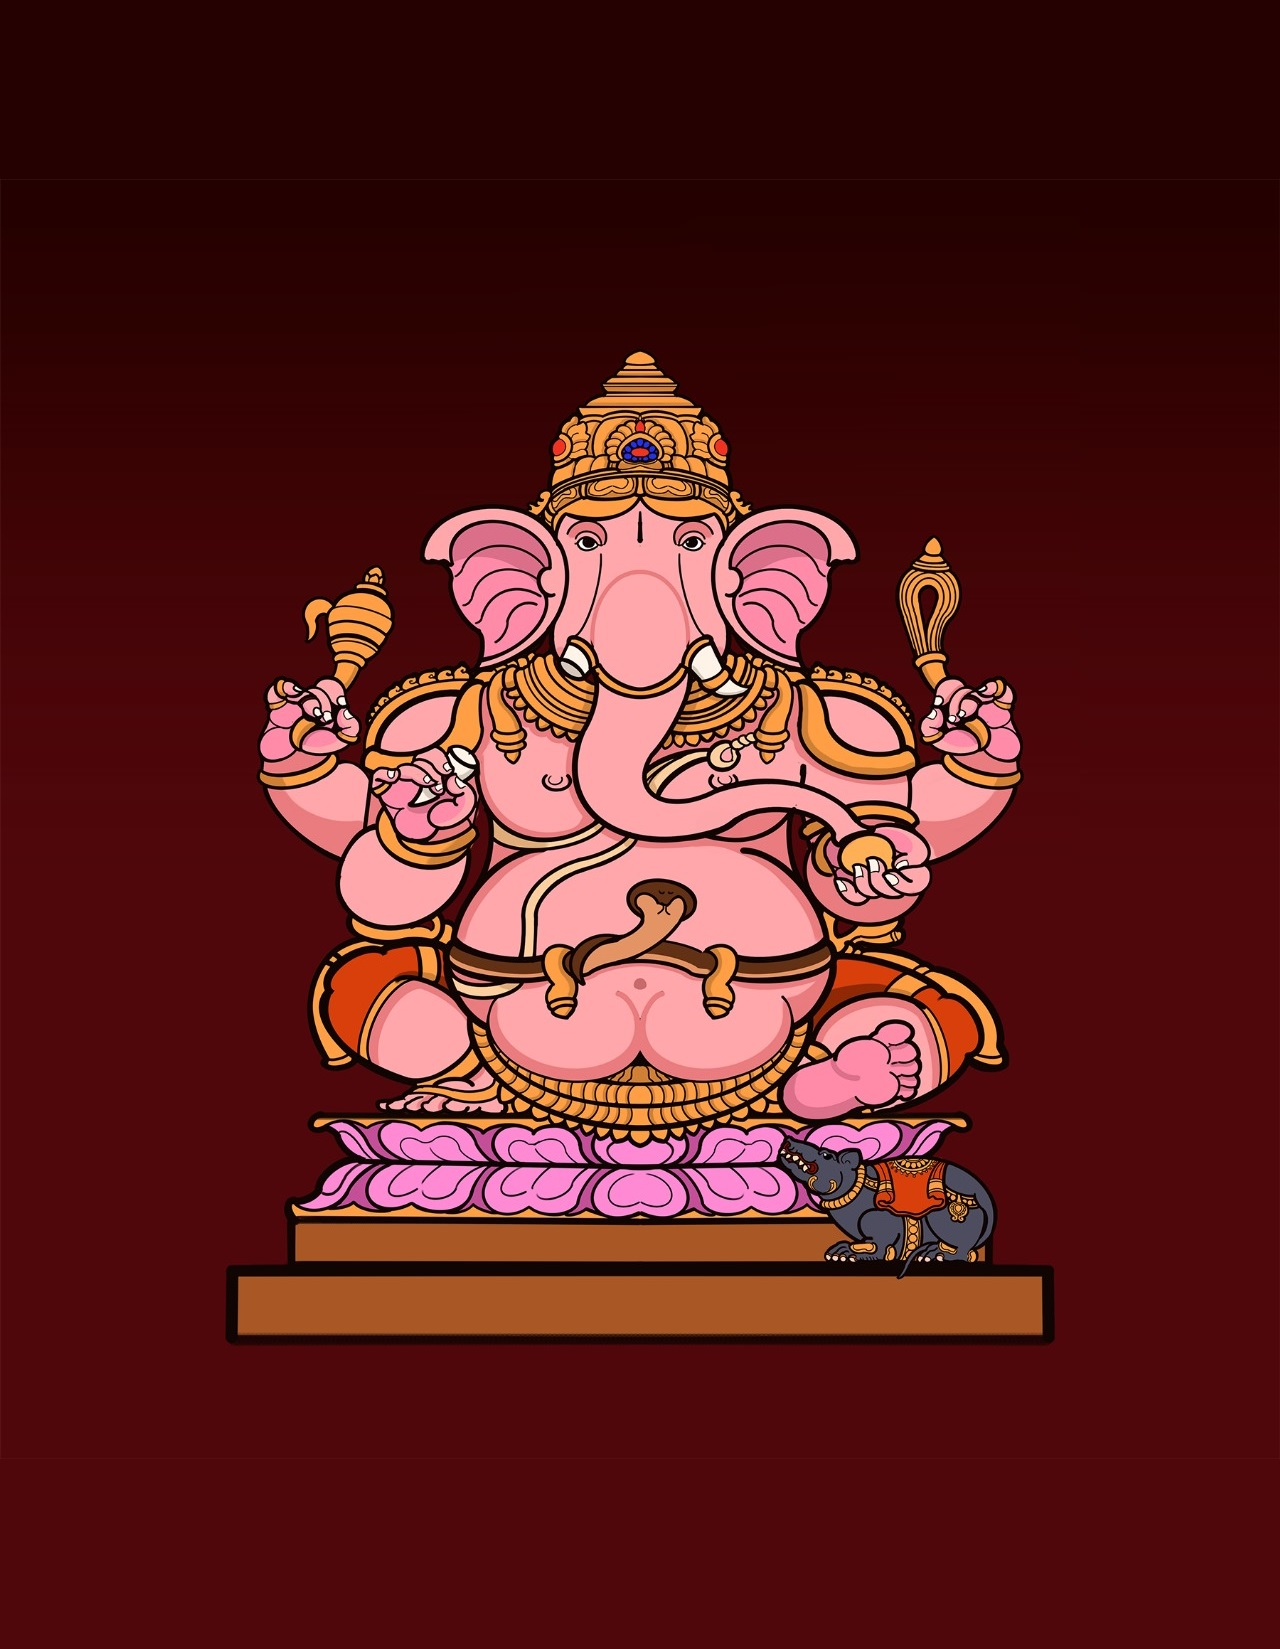
\includegraphics[width=0.9\textwidth, height=\paperheight, keepaspectratio]{./images/ganapa.jpg}
%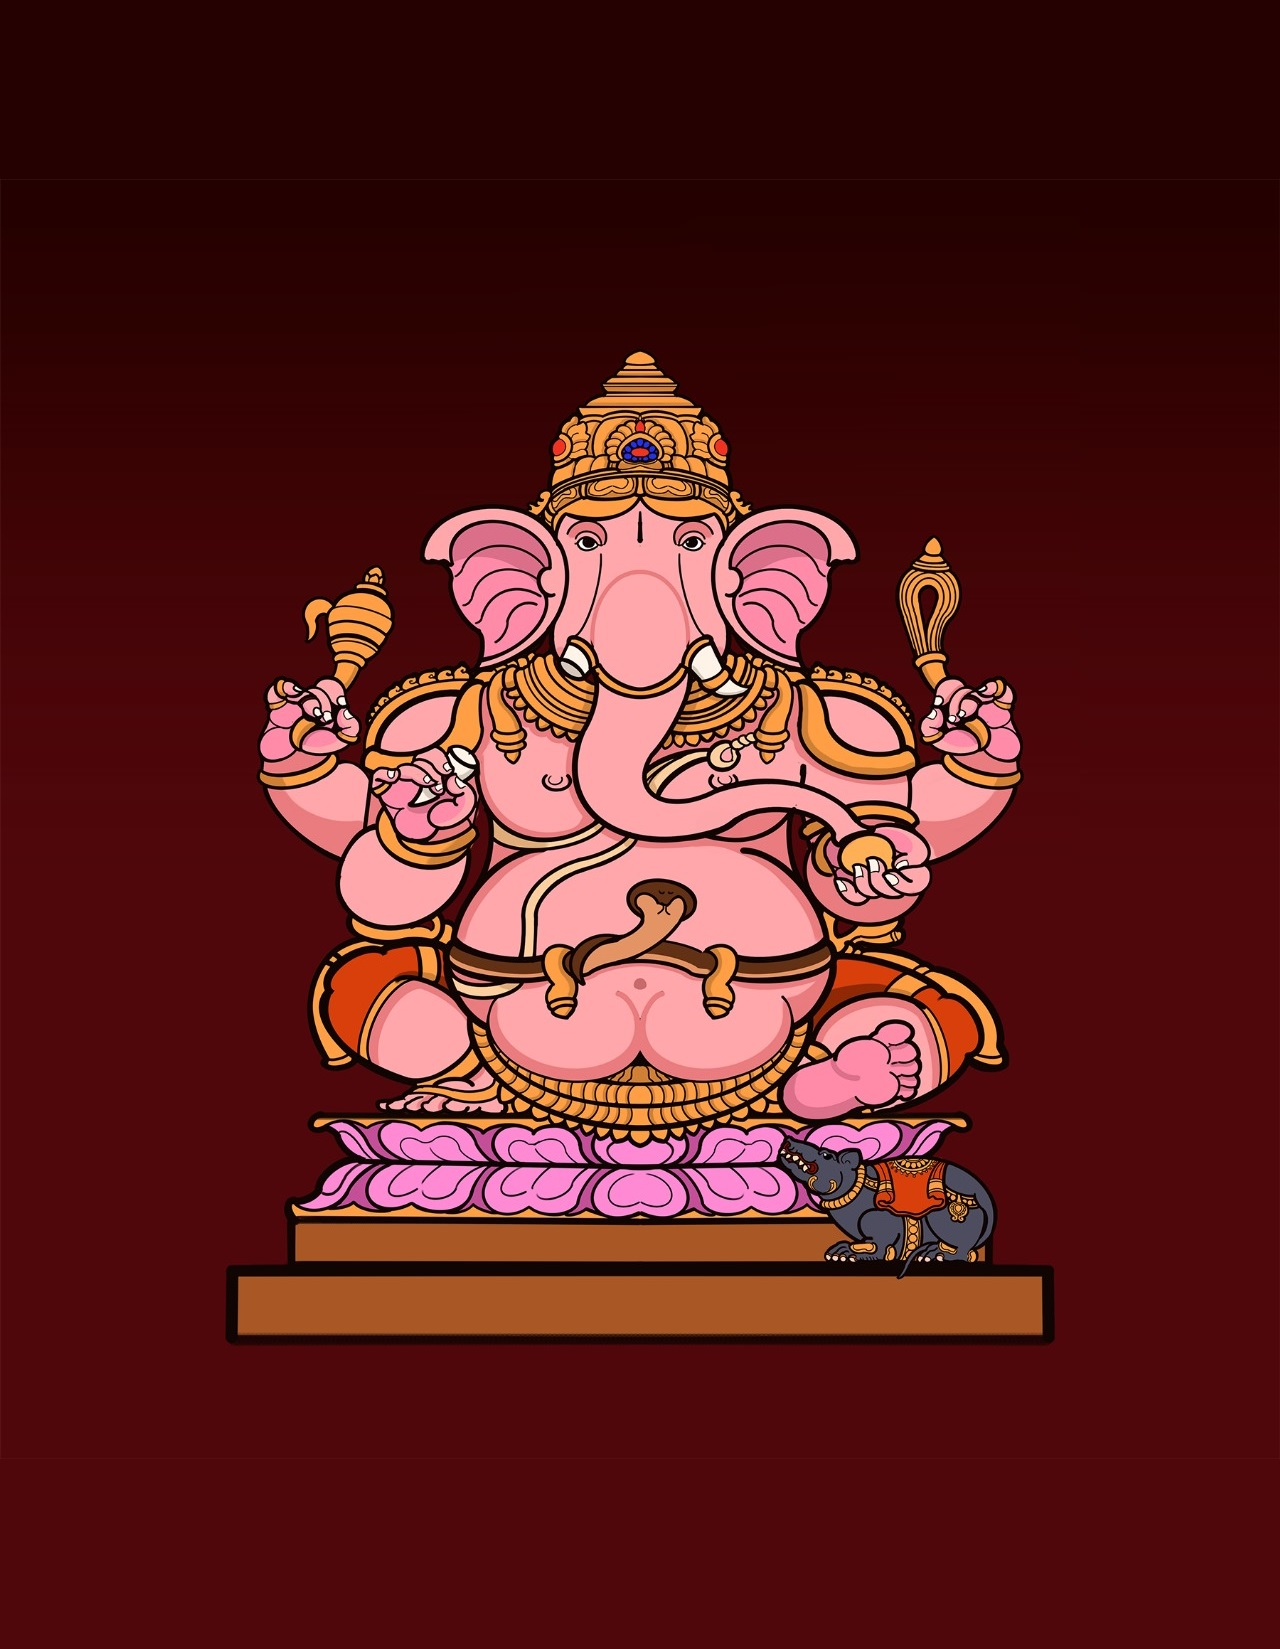
\includegraphics[width=\paperwidth, height=\paperheight]{./images/ganapa.jpg}
%\end{figure}
%\restoregeometry % Restore original geometry settings
%\newpage

\begin{figure}[h!]
    \centering
    \begin{overpic}[width=\paperwidth, height=\paperheight]{./images/001.jpg}
        \put(13,85){\color{white}\kanfont ಗಜಾನನಂ ಭೂತಗಣಾದಿ ಸೇವಿತಂ ಕಪಿತ್ಥ ಜಂಬೂಫಲಸಾರ ಭಕ್ಷಿತಮ್। }\put(10,82){\color{white}\kanfont ಉಮಾಸುತಂ ಶೋಕ ವಿನಾಶಕಾರಣಂ ನಮಾಮಿ ವಿಘ್ನೇಶ್ವರ ಪಾದಪಂಕಜಮ್॥ }
    \end{overpic}
    \caption{This is the standard figure caption below the image.}
    \label{fig:example}
\end{figure}

\restoregeometry
